
\begin{frame}
  \frametitle{Un visualisateur de fichier DVI accéléré par GPU}
  \begin{textblock}{2}(13,6.5)
    
\includegraphics[width=2cm]{images/ctan-lion.pdf}
  \end{textblock}
  % \begin{tikzpicture}[remember picture, overlay] run twice
  %   \node at ($(current page.south east) - (5cm,5cm)$) {
\includegraphics[width=2cm]{images/ctan-lion.pdf}};
  % \end{tikzpicture}
  \begin{center}
    \href{https://github.com/FabriceSalvaire/PyDVI}{PyDVI} a Python library to read and process DVI files
    % une bibliothéque Python pour lire et ... des fichiers DVI
  \end{center}
  % \vspace{5mm}
  \begin{columns}
    \begin{column}{.5\textwidth}
      \begin{itemize}
        \item packed font, Type 1, virtual font
        \item TeX font metric, Adobe Font Metrics
        \item font map
        \item font encoding
      \end{itemize}
      \vspace{1em}
      \begin{itemize}
      \item DVI $\longrightarrow$ PNG tool
      \item OpenGL Viewer
      \end{itemize}
    \end{column}
    \begin{column}{.5\textwidth}
      \begin{center}
        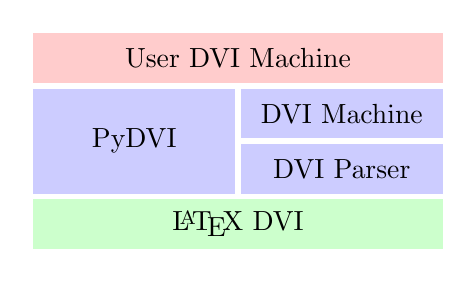
\begin{tikzpicture}[%
          base/.style={rectangle, minimum width=15em, minimum height=2em, draw=white, line width=2pt, anchor=south west},
          demibloc/.style={base, minimum width=7.5em}]
          \node[base, fill=green!20] at (0,0) {\LaTeX{} DVI};
          \node[demibloc, minimum height=4em, fill=blue!20] at (0,2em) {PyDVI};
          \node[demibloc, fill=blue!20] at (7.5em,2em) {DVI Parser};
          \node[demibloc, fill=blue!20] at (7.5em,4em) {DVI Machine};
          \node[base, fill=red!20] at (0,6em) {User DVI Machine};
        \end{tikzpicture}
      \end{center}
    \end{column}
  \end{columns}
  \vspace{1cm}
  \begin{center}
    \url{https://github.com/FabriceSalvaire/PyDVI}
  \end{center}
\end{frame}

%%% Local Variables: 
%%% mode: latex
%%% TeX-master: "master"
%%% End: 
